\chapter{Theoretical Background \& Literature Review}
\label{chap:two}
 
 As mentioned, this reports main focal point will be on the design of a \acs{LNA} front-end for a transducer utilizing a type of platinum-iridium based electrodes. 
 As such we will start exploring basic characteristics of neural signals and some practicalities on recording them, before we dig into the electronics theory necessary for us to determine a design methodology for the neural interface front-end. Notice also that remarks about the amplifier design - which is to be fully introduced in later chapters, are made as the theory discussion progresses.
 
  \section{Neural Recording through Biopotential Acquisition}
  \label{sec:biopotential-aquisition}
  Neural recording devices basically performs biopotential acquisition using transducers that converts ionic conduction to electronic conduction so that biopotential 
  signals can be stored and viewed. The biopotential signals themselves are generated due to electrochemical activity of electrogenic cells\footnote{\emph{Electrogenic cells} 
  refers to cells that exhibit the ability to generate electrical signals\cite{GBM8320-2013-electrodes-ch8-pt1}} - such as neurons, that are components of muscular, 
  nervous or glandular tissue. There are several measurement variations that are relevant for collecting biopotential data, whereas the ones considered most relevant 
  for the scope of this report are \emph{\acf{EEG}}, \emph{\acf{ECoG}} and \emph{\acf{iEEG}} (also commonly referred to by the somewhat misleading term \emph{\acf{LFP}}).
  
    From a historical perspective one usually refers to surface recording - that is, placing electrodes on top of the scalp - as \acs{EEG}, while \acs{ECoG} and \acs{iEEG} have coined the use of in-vivo
  intercranial electrodes in order to record electrical activity in the brains cerebral cortex\footnote{The \emph{cerebral cortex} is the outermost sheet of neural tissue covering the cerebral hemispheres in mammals. \cite{marcus2014future}}.
	More specifically on in-vivo recording; \acs{iEEG}\textbackslash\acs{LFP} is usually referred to when recordings are performed using small electrodes placed directly into the cortex from beneath the skull,
  while with \acs{ECoG} recordings one places the electrodes on the surface of the cortex.%\\*  
  
  
    \subsection{The Neural Signals}
     \label{subsec:neural-signals}
    We have have explained that there exists multiple measurement types for recording cortical activity. Biopotential signals generated by electrogenic cells like neurons, produce voltage changes on the order of 100 mV relative to the extracellular fluid \cite{kandel2000principles}. Collecting measurements of this type is possible in brief periods of time by carefully directing individual placement of microelectrodes intracellularly\footnote{\emph{Intracellular} means "inside the cell"}. To get around the limitations of only detecting single cells at a time - and for such short durations, the prime methodology at present is using microelectrode arrays extracellularly (though there exists rudimentary initiatives to merge the advantages of extracellular microelectrode arrays and intracellular microelectrodes, they have still not gained significant usability) \cite{spira2013multi}. A trade-off here is that we accept "blindness" to potentials generated by single cells as well as a significant reduction in signal amplitude. However, an interesting relationship is shown in figure %--------------------------figure-------------------------------------------------------------------        
    \begin{wrapfigure}{r}{4.5cm}
      \vspace{-20pt}
      \caption{\texttt{\footnotesize{Rec. of action potential}}}
      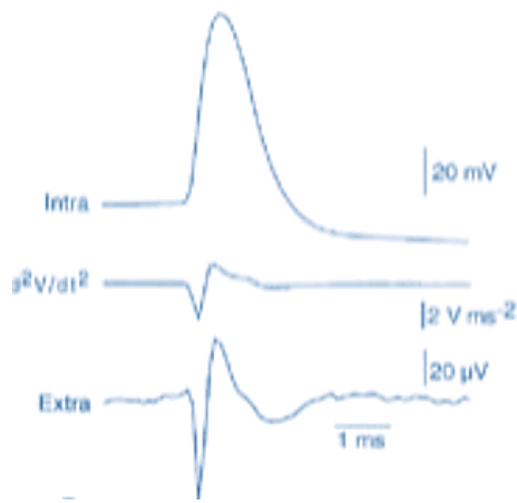
\includegraphics[width=4.5cm]{images/intracellular-amp-vs-extracellular-amp.png}
      \vspace{-25pt} 
      \label{fig:intracell-vs-extracell}
    \end{wrapfigure}
%--------------------------END-------------------------------------------------------------------
\ref{fig:intracell-vs-extracell} (adapted from \cite{extracell-action-pot-2009}); we can see that the shape of the extracellular voltage potential qualitatively matches the second time derivative of the intracellular voltage potential \cite{cohen2000contributions}. Note that the resulting variation in cellular potential with time is known as the action potential \cite{GBM8320-2013-electrodes-ch8-pt1}. Action potentials can be interpreted as "digital" events  - neurons normally induce spikes of similar amplitudes and time durations, and information is said to be found in the timing of these "digital" events \cite{harrison2008design}.
    
    A measurement type can be characterized by their signal strength (which we can see from fig.\ref{fig:cortical-measurements} is usually in the $\mu$-volts range) and surgical invasiveness 
    versus frequency and electrode area. This is presented in figure \ref{fig:cortical-measurements}.   
%--------------------------figure-------------------------------------------------------------------        
      \begin{figure}
	\centering
	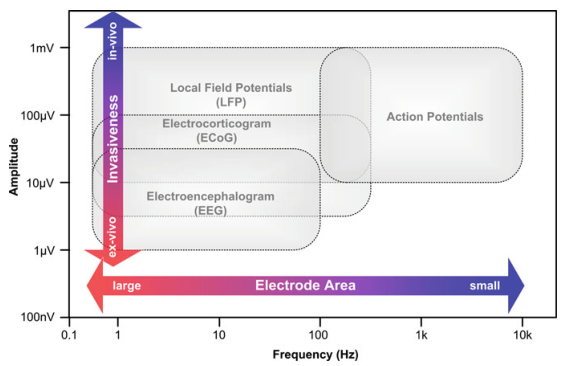
\includegraphics[scale=.75]{images/Amp-vs-freq-common-biopotential-signals2.png}
	\caption{\texttt{\footnotesize{different cortical measurements \cite{yoo2011biomedical-cmos}}}}
	\label{fig:cortical-measurements}
      \end{figure}
%--------------------------END-------------------------------------------------------------------
    \acs{ECoG} signals is measured using subdural surface electrodes (refer to 1. on fig.\ref{fig:neural-probe}). This type of measurement is outside of our design scope due to frequency range,
    but it can be mentioned that the method offers significant increase in spatial and temporal resolutions as well as stronger amplitudes - especially in 
    the high gamma frequency range\footnote{Gamma frequency ranges between ~70Hz to ~110Hz\cite{hill2012recording}}, 
    in contrast to the non-invasive surface based \acs{EEG} topologies \cite{hill2012recording}. This leads us to the very similar \acs{LFP} signals.
    \acs{LFP} oscillations differs from \acs{ECoG} in that LFPs are recorded from within the cortical tissue (illustrated by 2. in fig.\ref{fig:neural-probe}). 
    It is considered the internal correlate of \acs{ECoG} as it registers as the same "crowd noise" - that is synchronous activity of many neurons in one region of the brain,
    as ECoG recording, only with substantial blurring and attenuations. The signal deterioration happens because LFP oscillations is usually measured using microelectrode arrays \cite{harrison2008design}. This means LFP spectra is unavoidably detected with microelectrode arrays, even though one might only be after action potentials. It is, however, often beneficial to record both LFP together with action potential spikes and then apply linear filtering - which should be fairly easy to achieve considering frequency ranges are mostly different for the two signal types. LFPs are interesting for the same reasons that ECoG signals are; they have among other things been especially suitable in understanding motor movements of the body \cite{donoghue1998neural} and are consequently very suitable for e.g. neuroprosthetic applications.
    
    We notice from figure \ref{fig:cortical-measurements} that the low frequency characteristics and small signal amplitudes poses strict 
    noise requirements on designing a \acl{LNA}. In addition we know that \acs{CMOS} low noise design at such low frequencies will not
    be a straightforward experience because of \acs{CMOS} circuitry's susceptibility to flicker noise. For the \acs{LNA} design - which is to be introduced
    next chapter, we will focus on action potential measurements. Therefore flicker noise should be a little less of a problem for us as we are in the 100 Hz to 10 kHz 
    frequency range. We will however, have to deal with a larger impedance because smaller electrode area is needed to measure action potentials.
    Also an important remark to make is about eventual LFP signals; as it is assumed that our LNA will be used for interfacing with a microelectrode array, LFP parts ($<$ $\approx$200 Hz) in the recording
    would be amplified and they would have be filtered out at a later stage in the system if they are unwanted.
    
    Fig.\ref{fig:cortical-measurements} also tells us something of what \acf{CMRR} we have to expect from the LNA. Again we focus on action potentials and see that the frequency of interest is higher than e.g. the mains frequency for instance, so we can have a much more relaxed \acs{CMRR} than any other type of neural recording. We still need to try to minimize capacitive and inductive interferences though. In addition; tethering forces introduced by conductors will cause problems for electrodes inserted into the sensitive tissue of the brain. Therefore one should ideally place the amplifier as close to - ideally directly attached to, the transducer. A guideline summary of LNA design considerations in regards to what type of neural signal one seek to record is given in \cite{yoo2011biomedical-cmos} and illustrated in figure \ref{tab:lna-design-considerations}.
%--------------------------figure-------------------------------------------------------------------      
    \begin{figure}
      \centering
      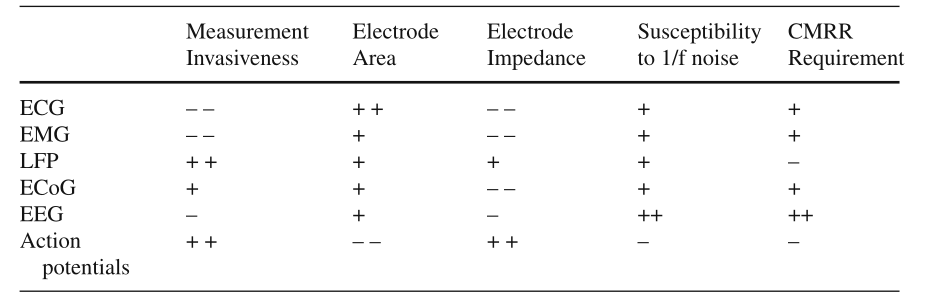
\includegraphics[scale=.5]{images/table-LNA-design-considerations.png}
      \captionsetup{singlelinecheck=off}
      \caption[\texttt{\footnotesize{LNA design considerations}}]{\texttt{\footnotesize{Summary of the considerations during the design of instrumentation amplifiers for different neural signals.\\
					      (-) indicates a low/small value \\
					      (+) indicates a high/large value}}}
      \label{tab:lna-design-considerations}
      \end{figure}
%--------------------------END-------------------------------------------------------------------              
       
    \subsection{Real-life Application of ideal Polarizable \& Non-Polarizable Electrodes} %%refer 4.2 in bimedical cmos
    \label{subsec:electrodes}
    To be able pick up biopotential-signals, current should flow from the tissue into the acquisition electronics. As the current is carried by ions in the body of a living being, a transducer is needed to convert ionic current into electronic current.\\*\\*
    Enter the \textbf{electrode}.\\ %See figure \ref{fig:neural-probe}\\
%--------------------------figure-------------------------------------------------------------------
    \begin{wrapfigure}{r}{0.5\textwidth}
      \centering
      \vspace{-20pt}
      \caption{\texttt{\footnotesize{electrode model}}}
      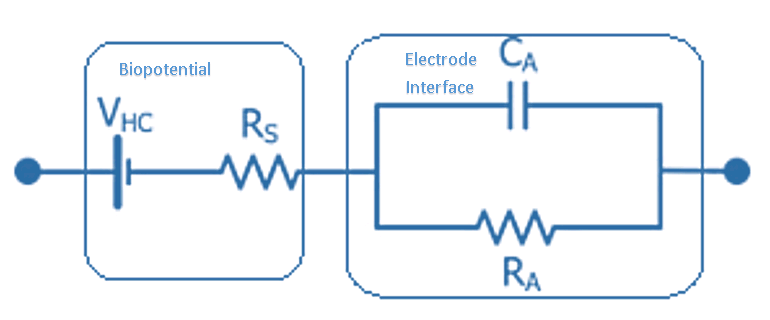
\includegraphics[width=0.5\textwidth]{images/electrical-probe-model1.png}
      \vspace{-35pt}
      \label{fig:probe-model}h
    \end{wrapfigure}
    \begin{wrapfigure}{r}{0.5\textwidth}
      \centering
      \vspace{-20pt}
      \caption{\texttt{\footnotesize{electrode array model}}}
      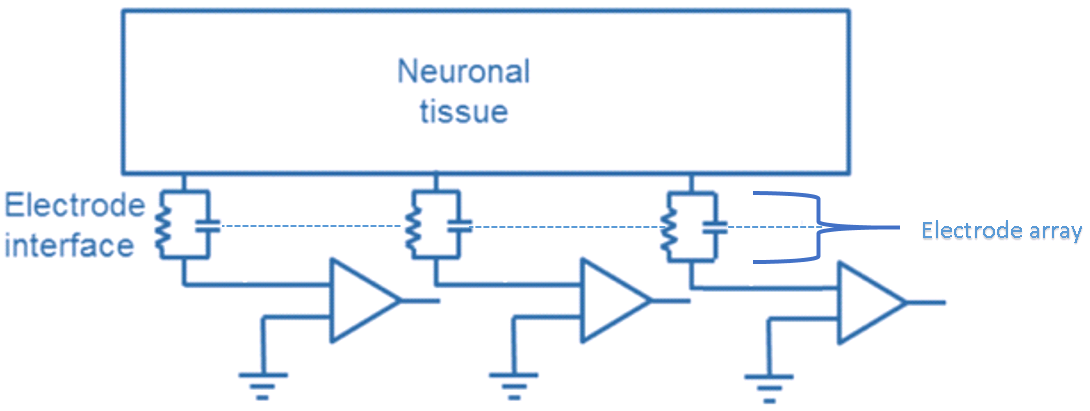
\includegraphics[width=0.5\textwidth]{images/electrical-probe-model-arrays.png}
      \vspace{-20pt}
      \label{fig:probe-model-array}
    \end{wrapfigure}
%--------------------------END-------------------------------------------------------------------  
    How easily electrons travel through the electrode interface defines if the electrode is considered non-polarizable or polarizable. If current flow 
    happens by very little energy, the electrode is referred to as being non-polarizable.  As such the electrode would ideally see no over-potentials and 
    thus, a \emph{perfectly} non-polarizable electrode can be seen as a simple resistor. If no charge crosses the electrode transfer, the electrode is 
    referred to as polarizable and can ideally be seen as capacitor as we only have a displacement current.
%--------------------------figure-------------------------------------------------------------------      
    \begin{figure}
      \centering
      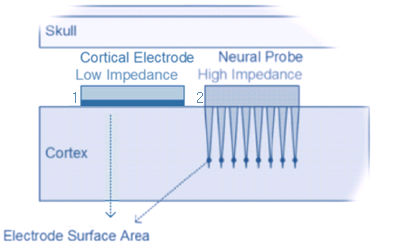
\includegraphics[scale=.7]{images/probe-placement2.png}
      \captionsetup{singlelinecheck=off}
      \caption[\texttt{\footnotesize{neural probe placement}}]{\texttt{\footnotesize{       				    
						    \begin{enumerate}
						      \item Cortical or subdural electrode placed under the skull directly on the surface of the brain.
						      \item Neuro-probe array placed on the surface of a brain. The recording electrodes are drawn as dots on the array of probes penetrating the cortex
						    \end{enumerate}}}}
      \label{fig:neural-probe}
      \end{figure}
%--------------------------END------------------------------------------------------------------- 
    However, the real world is not so forgiving; no electrode is purely polarizable or non-polarizable, rather something in between. We therefore present a 
    basic electrical model of a single electrode \cite{GBM8320-2013-electrodes-ch8-pt1} shown in figure \ref{fig:probe-model}.
    We see from \ref{fig:probe-model} that the source impedance can be modeled by a Thevenin equivalent source with a source impedance of Rs, while the electrode can be 
    modeled by a capacitor C\textsubscript{A} in parallel with a resistor R\textsubscript{A}.   
 
    Notice from figure \ref{fig:neural-probe} how the different electrode placement generally cover different areas. The impedance of an electrode plays an 
    important role during the design of the recording circuit when selecting amplifier design topology. We know that as the electrode surface 
    area decreases, its impedance tends to increase \cite{yoo2011biomedical-cmos}. Thus, the use of probes with high small electrode area
    forces us to design an amplifier with high input impedance.
   
   
   \section{MOSFET Based Amplifiers}\label{subsec:trans-amp-basics}
    
      \subsection{Designing Low-Noise and Low-Power \acs{OTA}s}
	%TODO:
	A major drawback in the classical amplifier design topology - e.g. operating transistors in strong inversion, arises from the fact that transistors in the active region limits a circuits power efficiency. As low-power 
	is critical in a neural recording front-end, an idea is to make sure transistors (mainly referring to the input pair the differential stage) operates in weak inversion. Now, as opposed to $g_m$ being proportional to the square 
	root of the drain current, the transconductance $g_m$ will be proportional to the drain current \cite{harrison2003low} which gives a better power efficiency. Maximizing $g_m$ in this way will also minimize 
	thermal noise in any CMOS differential amplifier \cite{johns2008analog} (note that we are aiming for a fixed drain current). Thus, the input pairs in the differential stage  will need  to  have a  large  W/L  ratio. However, 
	their length should ideally be as small as possible so that their width also is as small as possible. This way the input capacitance of the LNA does not become problematically large.
	
	From this we see that the sizing of our transistors are critical in maintaining a low-noise low-power design.
	\subsubsection{Level of Inversion}\label{subsubsec:lev-of-inv}
	As low-power also implies low-current; in addition to weak inversion operation
	we may have transistors working in moderate and strong inversion as well. As such it makes sense to define some tools which helps us use a transistors' level of inversion as a design variable
	and hence replace the conventional approaches involving the bias current and MOSFET channel widths.
	In this context, it would be prudent to introduce the inversion coefficient (IC) relationship - sometimes also refered to as level of inversion ratio:
	    \begin{equation} 
	    \label{eq:IC}
	      IC=I_D/I_S;
	    \end{equation}
	where the inversion characteristics current $I_S$ is given by
	    \begin{equation} 
	    \label{eq:inv-char-current}
	      I_S= \frac{2 \mu C_{ox} V_t^2}{ \kappa } \cdot W/L;
	    \end{equation}
	In equation \ref{eq:inv-char-current}, $\kappa$ would be the gate coupling coefficient in subthreshold operation, $V_t$ the thermal voltage, $C_{ox}$ the gate capacitance per unit area, and $\mu$ the mobility of electrons near the silicon surface. Lastly W and L is the transistor width and length respectively. We note that \cite{harrison2003low} claims $\kappa$ to have a typical value of $\sim$0.7. Returning to the inversion coefficient, the same 
	source tells us that IC gives us an understanding of a transistor operating region. That is, IC equates to\footnote{Notice that $\kappa = \frac{1}{n}$ where $n$ is called the subthreshold swing coefficiant (or ideality factor) and is the reciporal of the rate of change in the channel surface potential as a function of gate voltage \cite{kursun2006multi}}
		  \begin{itemize}
    		    \item strong inversion if IC$>$10;% ($V_{GS}>V_{TH}-100mV$);
    		    \item medium inversion if 10$>$IC$>$0.1; %($V_{TH}+100mV>V_{GS}>V_{TH}-100mV$);
    		    \item weak inversion if IC$<$0.1;% ($V_{GS}<V_{TH}-100mV$);
		  \end{itemize}
	This nicely contrasts the classical way of describing operating point in terms of gate-source voltage ($V_{GS}$).
	\subsubsection{Finding $g_m$ using IC and the EKV-model}\label{subsec:maxim-gm-EKV-model}
	In 1995 \cite{enz1995analytical} proposed a MOSFET-model valid for all operating points by deriving asymptotes for each operating point and linking them together using interpolation functions.
	This proposal is today being further developed as the EKV-model. They give the following equation for drain current
	    \begin{equation} \label{eq:Id-EKV}
	      I_D= I_S[ln(1 + \exp{\frac{\kappa (V_G-V_{TH})-V_S}{2V_T}})]^2;
	    \end{equation}
	where the $I_S$ is the same as before and $V_S$ is the source voltage of the transistor.
	We should remark that the original expression for calculating transconductance derived in \cite{enz1995analytical} is not cited here as it cannot be solved to find IC as a function of transconductance and drain current - which we need in order to maximize $g_m$.
	Instead we use the following interpolation function - as suggested by \cite{EE5720-Harrison-subtreshold}, to find the transconductance
	    \begin{equation} \label{eq:gm-EKV}
	      g_m= \frac{\kappa I_D}{V_t} \cdot \frac{2}{1+ \sqrt{1+4IC}};
	    \end{equation}	
	The EKV-model is said to be very helpful in low-power circuit design\cite{harrison2003low} and submicron and nanometer bulk-referenced applications\cite{shaoxi2010mosfet}.
      
	  
	 
	   
	   
      \subsection{Noise Performance}
	\subsubsection{Noise Figure}
%    	\[f_{DAC} = f_{HFPERCLK}  \frac{1}{2^{PRESC}}\]
        
%        bla bla bla derp dahsd
%        \begin{gather}
%        \label{cycle-formula}
%            \Delta C = \frac{f_{HFCORECLOCK}}{f_{samplerate}} = \frac{14000000}{44100} \approx 317
%        \end{gather}
%        tralalalla halo aodhnag
        
	\subsubsection{Noise Efficiency Factor}
	%TODO:
	In order to be able to compare the noise specifications
reached with other recently published IAs, a noise efficiency factor (NEF) is introduced. The total equivalent
input noise of an ideal bipolar transistor (only thermal
noise and no base resistance) is given by

2015HoST Project noise noiseEffFactor

with BW being the frequency bandwidth (for a bipoku
transistor this is the ft). The NEF of a system is then
defined as

2015HoST Project noise noiseEffFactor

where In, is the total current drain in the system and

Vi. is the total equivalent input noise. The NEF describes how many times the noise of a system with the
same current drain and bandwidth is higher compared to
the ideal case, e.g., for a CMOS transistor with only white
noise, the noise power is given by

2015HoST Project noise noiseEffFactor

  